
\begin{center}
    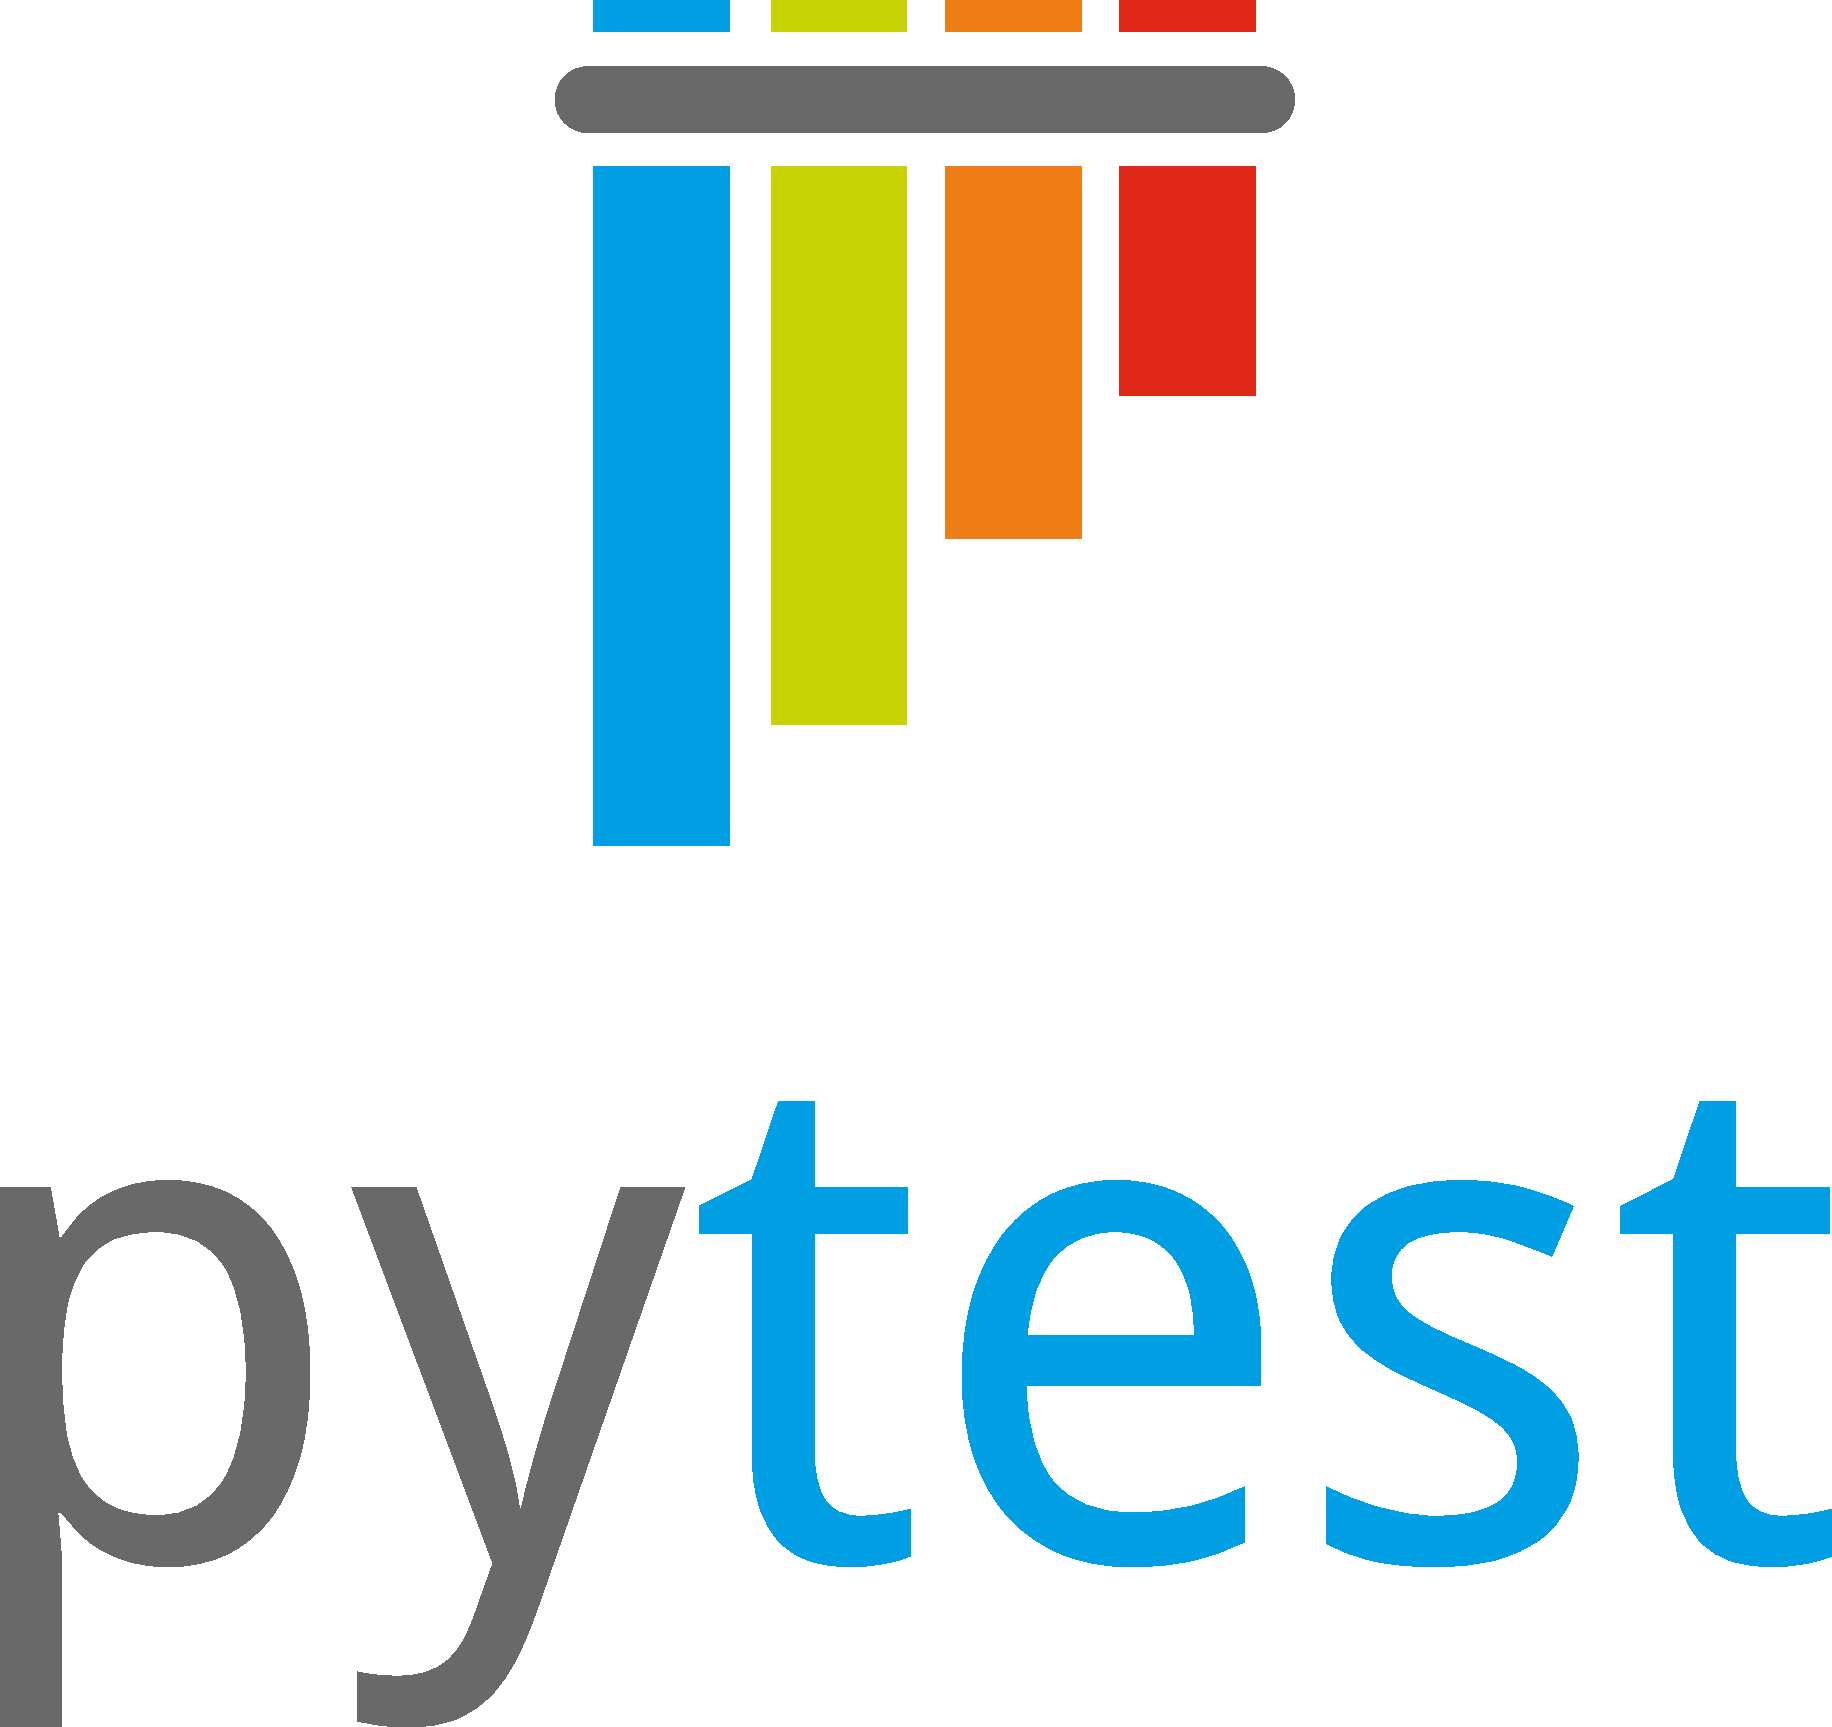
\includegraphics[width=.5\linewidth]{img/pytest.pdf}
    \vspace{1.25em}

    {\Huge Quick Reference} \\
    \vspace{2em}
    {\huge by}
    \vspace{.75em}

    
\includegraphics[width=.8\linewidth]{img/bruhinsw.pdf} \\

    \vspace{2.25em}
    {\color{codeblue}\hrule}
    \vspace{1em}

    \begin{minipage}{.2\linewidth}
        \vspace{2.5em}
        \textcolor{codeblue}{\qrcode[height=\linewidth]{https://bruhin.software}}
    \end{minipage}
    \hspace{.5em}
    \begin{minipage}{.75\linewidth}
        {\LARGE \bold{Level up your testing!}}
        \vspace{1em}

        \large
        Python / \bold{pytest trainings}, \\
        consulting and development by one of \bold{pytest's core maintainers}.
    \end{minipage}
\end{center}

\bold{Get a three-day deep-dive into testing with pytest:} \\[.25em]
Writing your first test, using fixtures, mocking, and even
writing your own plugins.

The training is designed to be interactive with \bold{hands-on exercises} and \bold{real-world examples}.

Tailored trainings are offered \bold{on-site} at your company (CH/DE/AT/\ldots{}) or \bold{remotely}.
\vspace{1.25em}

{\color{codeblue}\hrule}

\vfill
{%
    \small
    \faCreativeCommons{} \faCreativeCommonsBy{} \faCreativeCommonsNd{} \, CC BY-ND 4.0 \\
    \faCopyright[regular]{} \, 2026 Freya Bruhin \\[.5em]
    \faGithub{} \, The-Compiler/pytest-cheat-sheet \\
    \faEnvelope{} \, freya@bruhin.software
}
